% Options for packages loaded elsewhere
\PassOptionsToPackage{unicode}{hyperref}
\PassOptionsToPackage{hyphens}{url}
\PassOptionsToPackage{dvipsnames,svgnames,x11names}{xcolor}
%
\documentclass[
  letterpaper,
  DIV=11,
  numbers=noendperiod]{scrartcl}

\usepackage{amsmath,amssymb}
\usepackage{iftex}
\ifPDFTeX
  \usepackage[T1]{fontenc}
  \usepackage[utf8]{inputenc}
  \usepackage{textcomp} % provide euro and other symbols
\else % if luatex or xetex
  \usepackage{unicode-math}
  \defaultfontfeatures{Scale=MatchLowercase}
  \defaultfontfeatures[\rmfamily]{Ligatures=TeX,Scale=1}
\fi
\usepackage{lmodern}
\ifPDFTeX\else  
    % xetex/luatex font selection
\fi
% Use upquote if available, for straight quotes in verbatim environments
\IfFileExists{upquote.sty}{\usepackage{upquote}}{}
\IfFileExists{microtype.sty}{% use microtype if available
  \usepackage[]{microtype}
  \UseMicrotypeSet[protrusion]{basicmath} % disable protrusion for tt fonts
}{}
\makeatletter
\@ifundefined{KOMAClassName}{% if non-KOMA class
  \IfFileExists{parskip.sty}{%
    \usepackage{parskip}
  }{% else
    \setlength{\parindent}{0pt}
    \setlength{\parskip}{6pt plus 2pt minus 1pt}}
}{% if KOMA class
  \KOMAoptions{parskip=half}}
\makeatother
\usepackage{xcolor}
\setlength{\emergencystretch}{3em} % prevent overfull lines
\setcounter{secnumdepth}{-\maxdimen} % remove section numbering
% Make \paragraph and \subparagraph free-standing
\ifx\paragraph\undefined\else
  \let\oldparagraph\paragraph
  \renewcommand{\paragraph}[1]{\oldparagraph{#1}\mbox{}}
\fi
\ifx\subparagraph\undefined\else
  \let\oldsubparagraph\subparagraph
  \renewcommand{\subparagraph}[1]{\oldsubparagraph{#1}\mbox{}}
\fi


\providecommand{\tightlist}{%
  \setlength{\itemsep}{0pt}\setlength{\parskip}{0pt}}\usepackage{longtable,booktabs,array}
\usepackage{calc} % for calculating minipage widths
% Correct order of tables after \paragraph or \subparagraph
\usepackage{etoolbox}
\makeatletter
\patchcmd\longtable{\par}{\if@noskipsec\mbox{}\fi\par}{}{}
\makeatother
% Allow footnotes in longtable head/foot
\IfFileExists{footnotehyper.sty}{\usepackage{footnotehyper}}{\usepackage{footnote}}
\makesavenoteenv{longtable}
\usepackage{graphicx}
\makeatletter
\def\maxwidth{\ifdim\Gin@nat@width>\linewidth\linewidth\else\Gin@nat@width\fi}
\def\maxheight{\ifdim\Gin@nat@height>\textheight\textheight\else\Gin@nat@height\fi}
\makeatother
% Scale images if necessary, so that they will not overflow the page
% margins by default, and it is still possible to overwrite the defaults
% using explicit options in \includegraphics[width, height, ...]{}
\setkeys{Gin}{width=\maxwidth,height=\maxheight,keepaspectratio}
% Set default figure placement to htbp
\makeatletter
\def\fps@figure{htbp}
\makeatother

\KOMAoption{captions}{tableheading}
\makeatletter
\@ifpackageloaded{tcolorbox}{}{\usepackage[skins,breakable]{tcolorbox}}
\@ifpackageloaded{fontawesome5}{}{\usepackage{fontawesome5}}
\definecolor{quarto-callout-color}{HTML}{909090}
\definecolor{quarto-callout-note-color}{HTML}{0758E5}
\definecolor{quarto-callout-important-color}{HTML}{CC1914}
\definecolor{quarto-callout-warning-color}{HTML}{EB9113}
\definecolor{quarto-callout-tip-color}{HTML}{00A047}
\definecolor{quarto-callout-caution-color}{HTML}{FC5300}
\definecolor{quarto-callout-color-frame}{HTML}{acacac}
\definecolor{quarto-callout-note-color-frame}{HTML}{4582ec}
\definecolor{quarto-callout-important-color-frame}{HTML}{d9534f}
\definecolor{quarto-callout-warning-color-frame}{HTML}{f0ad4e}
\definecolor{quarto-callout-tip-color-frame}{HTML}{02b875}
\definecolor{quarto-callout-caution-color-frame}{HTML}{fd7e14}
\makeatother
\makeatletter
\@ifpackageloaded{caption}{}{\usepackage{caption}}
\AtBeginDocument{%
\ifdefined\contentsname
  \renewcommand*\contentsname{Table of contents}
\else
  \newcommand\contentsname{Table of contents}
\fi
\ifdefined\listfigurename
  \renewcommand*\listfigurename{List of Figures}
\else
  \newcommand\listfigurename{List of Figures}
\fi
\ifdefined\listtablename
  \renewcommand*\listtablename{List of Tables}
\else
  \newcommand\listtablename{List of Tables}
\fi
\ifdefined\figurename
  \renewcommand*\figurename{Figure}
\else
  \newcommand\figurename{Figure}
\fi
\ifdefined\tablename
  \renewcommand*\tablename{Table}
\else
  \newcommand\tablename{Table}
\fi
}
\@ifpackageloaded{float}{}{\usepackage{float}}
\floatstyle{ruled}
\@ifundefined{c@chapter}{\newfloat{codelisting}{h}{lop}}{\newfloat{codelisting}{h}{lop}[chapter]}
\floatname{codelisting}{Listing}
\newcommand*\listoflistings{\listof{codelisting}{List of Listings}}
\makeatother
\makeatletter
\makeatother
\makeatletter
\@ifpackageloaded{caption}{}{\usepackage{caption}}
\@ifpackageloaded{subcaption}{}{\usepackage{subcaption}}
\makeatother
\ifLuaTeX
  \usepackage{selnolig}  % disable illegal ligatures
\fi
\usepackage{bookmark}

\IfFileExists{xurl.sty}{\usepackage{xurl}}{} % add URL line breaks if available
\urlstyle{same} % disable monospaced font for URLs
\hypersetup{
  pdftitle={Evidence for ecological niche partitioning among ribbon and spotted seals in the Bering Sea and implications for their resilience to climate change},
  pdfauthor={Josh M. London; Heather L. Ziel; Lorrie D. Rea; Stacie M. Koslovsky; Michael F. Cameron; Peter L. Boveng},
  colorlinks=true,
  linkcolor={blue},
  filecolor={Maroon},
  citecolor={Blue},
  urlcolor={Blue},
  pdfcreator={LaTeX via pandoc}}

\title{Evidence for ecological niche partitioning among ribbon and
spotted seals in the Bering Sea and implications for their resilience to
climate change}
\author{Josh M. London \and Heather L. Ziel \and Lorrie D.
Rea \and Stacie M. Koslovsky \and Michael F. Cameron \and Peter L.
Boveng}
\date{2024-03-27}

\begin{document}
\maketitle
\begin{abstract}
In deep-diving seals (\emph{Phocidae}) niche partitioning has been
observed as delineation in time, multi-dimensional use of the ocean, or
diet composition. Here, we focus on two species of seals in the Bering
Sea -- ribbon seals (\emph{Histriophoca fasciata}) and spotted seals
(\emph{Phoca largha}) -- and evidence for niche partitioning from two
decades of bio-logger deployments (n=110 ribbon; n=82 spotted) and
stable isotope sampling (n=29 ribbon; n=43 spotted). Whiskers of
dependent pups in the spring reflect the isotopic space of adult female
diet in the winter (when the pup was developing in-utero) and sampling
from the whisker base of adults in the spring corresponds with the
isotopic space of their recent diet. In both seasons, spotted seals had
higher mean δ13C (winter: +6.9\%; spring: +3.8\%) and δ15N (winter:
+10.5\%; spring = +12.1\%) values, which are reflective of on-shelf and
coastal foraging at a higher trophic level. Two-dimensional utilization
distributions (UD) were estimated from bio-logger geolocations for each
species during similar seasonal periods (`spring' and `fall-winter').
Optimally weighted auto-correlated kernel density estimates were
combined into a population UD to test spatial overlap. Greater overlap
was observed in the spring when both species rely on the marginal
sea-ice zone for pupping, breeding, and molting. More separation was
observed during the fall-winter season when spotted seals remained
largely on the continental shelf and ribbon seals shifted to the shelf
break and Bering Sea basin. Dive behavior records showed ribbon seals
consistently diving to deeper depths (max dive depth =
\textasciitilde600m) compared to spotted seals (max dive depth =
\textasciitilde300m) indicating additional partitioning of resources
within the water column. Changes in the extent and timing of sea ice in
the Bering Sea along with anomalous warming events could disrupt the
niche partitioning between these seal species and, thus, challenge their
resilience to climate change.

\begin{tcolorbox}[enhanced jigsaw, breakable, colbacktitle=quarto-callout-warning-color!10!white, colback=white, left=2mm, coltitle=black, opacityback=0, rightrule=.15mm, opacitybacktitle=0.6, arc=.35mm, toptitle=1mm, bottomrule=.15mm, titlerule=0mm, colframe=quarto-callout-warning-color-frame, leftrule=.75mm, bottomtitle=1mm, title={Under Development. Please do not cite or use}, toprule=.15mm]

Please note this analysis and manuscript is still in draft form and
under active development. Changes to results, code, and the manuscript
are likely and this should not be cited or used for any reason. We are
sharing the work and development of this manuscript in the spirit of
open science, improved transparency, and scientific reproducibility.

We plan to provide a preprint to bioRxiv prior to journal submission.

\end{tcolorbox}
\end{abstract}

\section{Introduction}\label{introduction}

\begin{itemize}
\tightlist
\item
  review definition of niche partitioning;
\item
  review of previous studies (terrestrial/marine) of niche partitioning
  that relied on evidence from stable isotopes, geo-locations from
  bio-loggers, OR, for marine animals, dive behavior;
\item
  highlight any studies that used an integrated approach (e.g.~stable
  isotopes and movement). any previous studies that integrated across
  all three?
\item
  review climate change impacts in the Arctic/Bering Sea and focus in on
  ribbon and spotted seals
\item
  previously published studies, observations, LTK(?), describing the
  ecology of ribbon and spotted seals that indicated potential for niche
  separation
\item
  study objectives:

  \begin{itemize}
  \tightlist
  \item
    Do stable isotope and bio-logging data from nearly 2 decades of
    research provide evidence for niche partitioning among ribbon and
    spotted seals?
  \item
    How might predicted climate change impacts in the Bering Sea affect
    this established partitioning of resources and will ribbon and
    spotted seals be resient to such change?
  \end{itemize}
\end{itemize}

\section{Methods}\label{methods}

\subsection{Stable Isotope Analysis}\label{stable-isotope-analysis}

Whiskers, hair, and blood (RBC and Plasma) from ribbon and spotted seals
of all age classes were collected in the field as part of larger
research efforts studying the ecology and health of ice-associated seals
in the Bering Sea. All samples were collected from live seals captured
in the spring (April-June) within the marginal ice zone at the southern
edge of sea-ice extent.

Stable isotope analysis was based on whiskers sampled from all age
classes (dependent pup, young of the year, subadult, adult) between 2009
and 2022. For all age classes, samples were taken along the length of
the whisker starting at the root. Samples further from the root
represent the isotopic space further back in time. Stable isotopes from
whiskers of dependent pups in the spring reflect the isotopic space of
adult female diets in the winter (when the pup was developing in-utero)
and sampling from the whisker base (segment 2) of adults in the spring
corresponds with recent isotopic use (when those tissues were
generated). Growth rates of whiskers in phocids are not linear and,
thus, we can't attribute a specific segment of the whisker to a specific
point in time -- except for the base segment near the root. Dependent
pups, however, offer a unique opportunity because we know the majority
of the whisker was developed in-utero and would represent the adult
female's forgaing during the preceding fall/winter. Once the pup starts
nursing, however, the trophic level changes and we can expect segments
nearest the root to reflect this. For this analysis we only consider
samples from the distant half of the whisker to most closely match the
in-utero period. We simply averaged those samples.

For comparison of the isotopic space, we used the R package, SIBER.

\subsection{Utilization Distributions from Bio-logger
Deployments}\label{utilization-distributions-from-bio-logger-deployments}

A total of 112 bio-loggers (SPLASH family, Wildlife Computers, Redmond,
Washington, USA) were deployed on 67 ribbon seals and 45 spotted seals
between 2005 and 2022. The deployments span all age classes with the
exception of dependent pups for both species and were deployed during
the months of April, May, and June. In some cases, deployments were
initiated prior to molting and the bio-loggers fell off after a period
of weeks to two months. Deployments initiated after molting transmitted
up to \textasciitilde9 months.

All deployments were checked for any data quality issues and
inconsistent location estimates before they were run through a course
speed filter to remove any locations that would have required a
sustained swim speed greater than 15 km/h. Additionally, any deployments
with fewer than 30 location estimates or a total deployment length less
than 7 days were removed. Lastly, to improve movement model fitting, we
thinned the location estimates to remove any time steps less than 10
minutes.

Two data sets for each species were created to include only movement in
the months of April, May, and June (`spring') and October, November, and
December (`open water'). The continuous time movement model used in the
analysis is stationary and predicated on a general range limitation to
the underlying movement behavior. Both species have known association
with the marginal sea-ice zone during the spring months as they focus on
pupping, breeding, and molting. The fall/winter months were chosen to
match the time duration of the spring period when the Bering Sea is
largely ice free. This period also coincides with the season when
in-utero development of pups that are sampled for stable isotope
analysis in the spring.

Utilization distributions were estimated for each species and each of
the seasonal periods based on a continuous time movement model (R
package \texttt{ctmm}). Specifically, optimally weighted auto-correlated
kernel density estimates (wAKDE) were created to reflect a more honest
account of space use while also mitigating sampling bias from irregular
deployment lengths. The weighted AKDE utilization distributions were
combined into a population kernel density estimate that should better
reflect spatial distribution of the broader population beyond just the
sampled seals.

\subsection{Dive Behavior From Bio-logger
Deployments}\label{dive-behavior-from-bio-logger-deployments}

\section{Results}\label{results}

\subsection{Stable Isotope}\label{stable-isotope}

(n = 7 ribbon; n = 31 spotted)

(n = 23 ribbon; n = 35 spotted)

The figures below show results from the initial stable isotope analysis
for pups sampled to represent adult female fall/winter foraging (figure
1) and for sub-adults and adults (figure 2) sampled to represent their
foraging close to the time of sampling (spring).

The plots show the values as well as a convex hull and an ellipse which
represents the 95\% confidence interval around the bivariate mean.

\begin{figure}[H]

{\centering 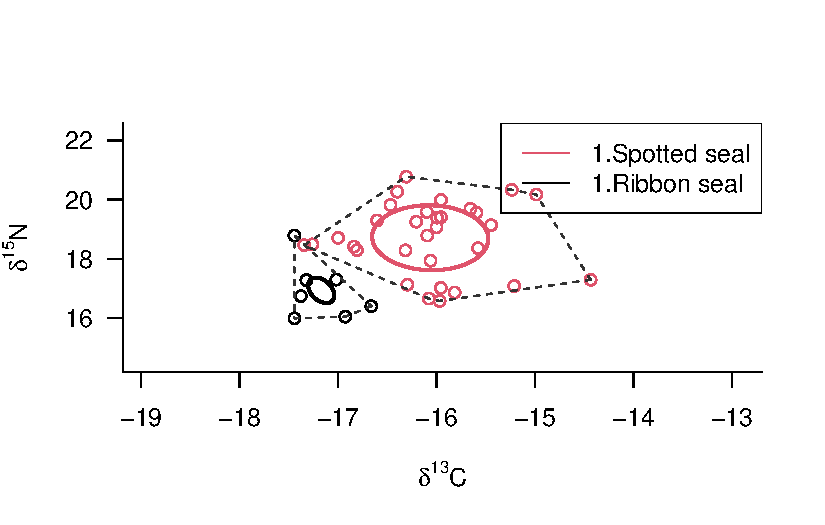
\includegraphics{index_files/figure-pdf/unnamed-chunk-15-1.pdf}

}

\caption{Isotopic space of ribbon and spotted seal adult females in
winter (sampled from dependent pup whiskers that developed in-utero)}

\end{figure}%

\textsubscript{Source:
\href{https://noaa-afsc.github.io/ribbon-spotted-niche-partition/index.qmd.html}{Article
Notebook}}

\begin{figure}[H]

{\centering 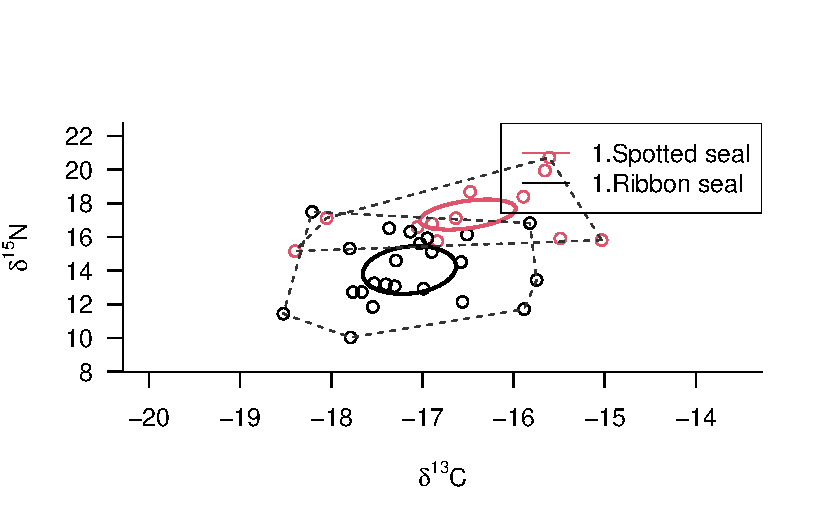
\includegraphics{index_files/figure-pdf/unnamed-chunk-16-1.pdf}

}

\caption{Isotopic space of ribbon and spotted seal adults and sub-adults
sampled from the root of the whisker sampled in the spring}

\end{figure}%

\textsubscript{Source:
\href{https://noaa-afsc.github.io/ribbon-spotted-niche-partition/index.qmd.html}{Article
Notebook}}



\end{document}
